Reproducing an experiment is a common practice by which scientists verify claims and apply new ideas to their 
own domain of study. Reproducible research saves a great amount of time and budget when another scientist picks 
a study and tries to recreate the same experiment. Overall, it avoids “reinventing the wheel.”

In the scientific community, the reproducibility concept is often approached from two different perspectives. 
Some researchers view it as a tool for verifying a claim. This approach is required when for example new 
findings are planned to be applied to real life problems. There is also a complementary perspective through 
which the scientists view reproducibility as a tool for improving an existing method, adapting it to new 
requirements and needs, or applying the methodology to a new domain of research.

Through recent years, along with the increase in the amount of data available to the scientific community, 
more high performance computational resources have also become accessible to researchers. The combination 
of these two, has led to both new discoveries and research opportunities while introducing new challenges. 
The traditional scientific paper of an experiment (being designed to include all the necessary information 
of a study) does not appear to be able to contain all the required information of the data-intensive and 
computationally-intensive methods of the modern studies. While it’s challenging to reproduce a study from 
scratch using the provided information on the study report, not having proper enough details, adds up to 
the problem and endangers the reproducibility of a claim for verification, adjustment or application purposes.

In an attempt to reproduce a paper on protein classification on an imbalance dataset (which is a common case 
in this domain) from the second perspective mentioned above, we obtained a wide range of results with the 
available details on the study report. The authors had shared a fair amount of details on the paper which 
does not seem to be enough for problems with an imbalanced dataset. In such problems, for predicting the final 
labels, a researcher needs to take some extra steps which involves more parameters throughout the whole process. 
We believe in similar problems, the study report should also include details on these important parameters to 
enable reproducibility.

In our study, we approach the methodological reproducibility of the classification problems with an imbalance 
dataset from the perspective mentioned above. We address the potential underlying reproducibility-related issues 
of the similar studies and how those could lead to a wide range of results in reproduction. In this section, we 
will briefly provide our adopted definition of some common reproducibility terms to further clarify the 
upcoming discussions.

\subsection{Taxonomy and Terms}

\subsubsection{Reproducibility}
The term “reproducibility” came about in the early 90s in computational science by John Claerbout and through the 
context of transparency. He provided a set of procedures on the paper allowing the reader to see the entire process 
from the data to figures and tables \cite{claerbout_electronic_1992}. The concept has been carried forward into 
other domains (e.g. bioinformatics, economics, etc) afterwards 
\cite{king_replication_1995,peng_reproducible_2006,schwab_making_2000}. since then and has been transformed into 
the context we use today.

In its modern context, the U.S. National Science Foundation (NSF) \cite{cacioppo_social_2015} defines reproducibility 
as “the ability of a researcher to duplicate the results of a prior study using the same materials as were used by 
the original investigator. That is, a second researcher might use the same raw data to build the same analysis files 
and implement the same statistical analysis in an attempt to yield the same results.” 

\subsubsection{Reproducibility, Replicability, Robustness and Generalizability}
For the Reproducible, Replicable, Robust and Generalizable studies, we adopt the following definitions 
from \cite{pineau_improving_2020}. A study is \textbf{reproducible} when the same results could be obtained using the same data, 
analytical tools and through the same environment.

\begin{figure}[ht]
    \centering
    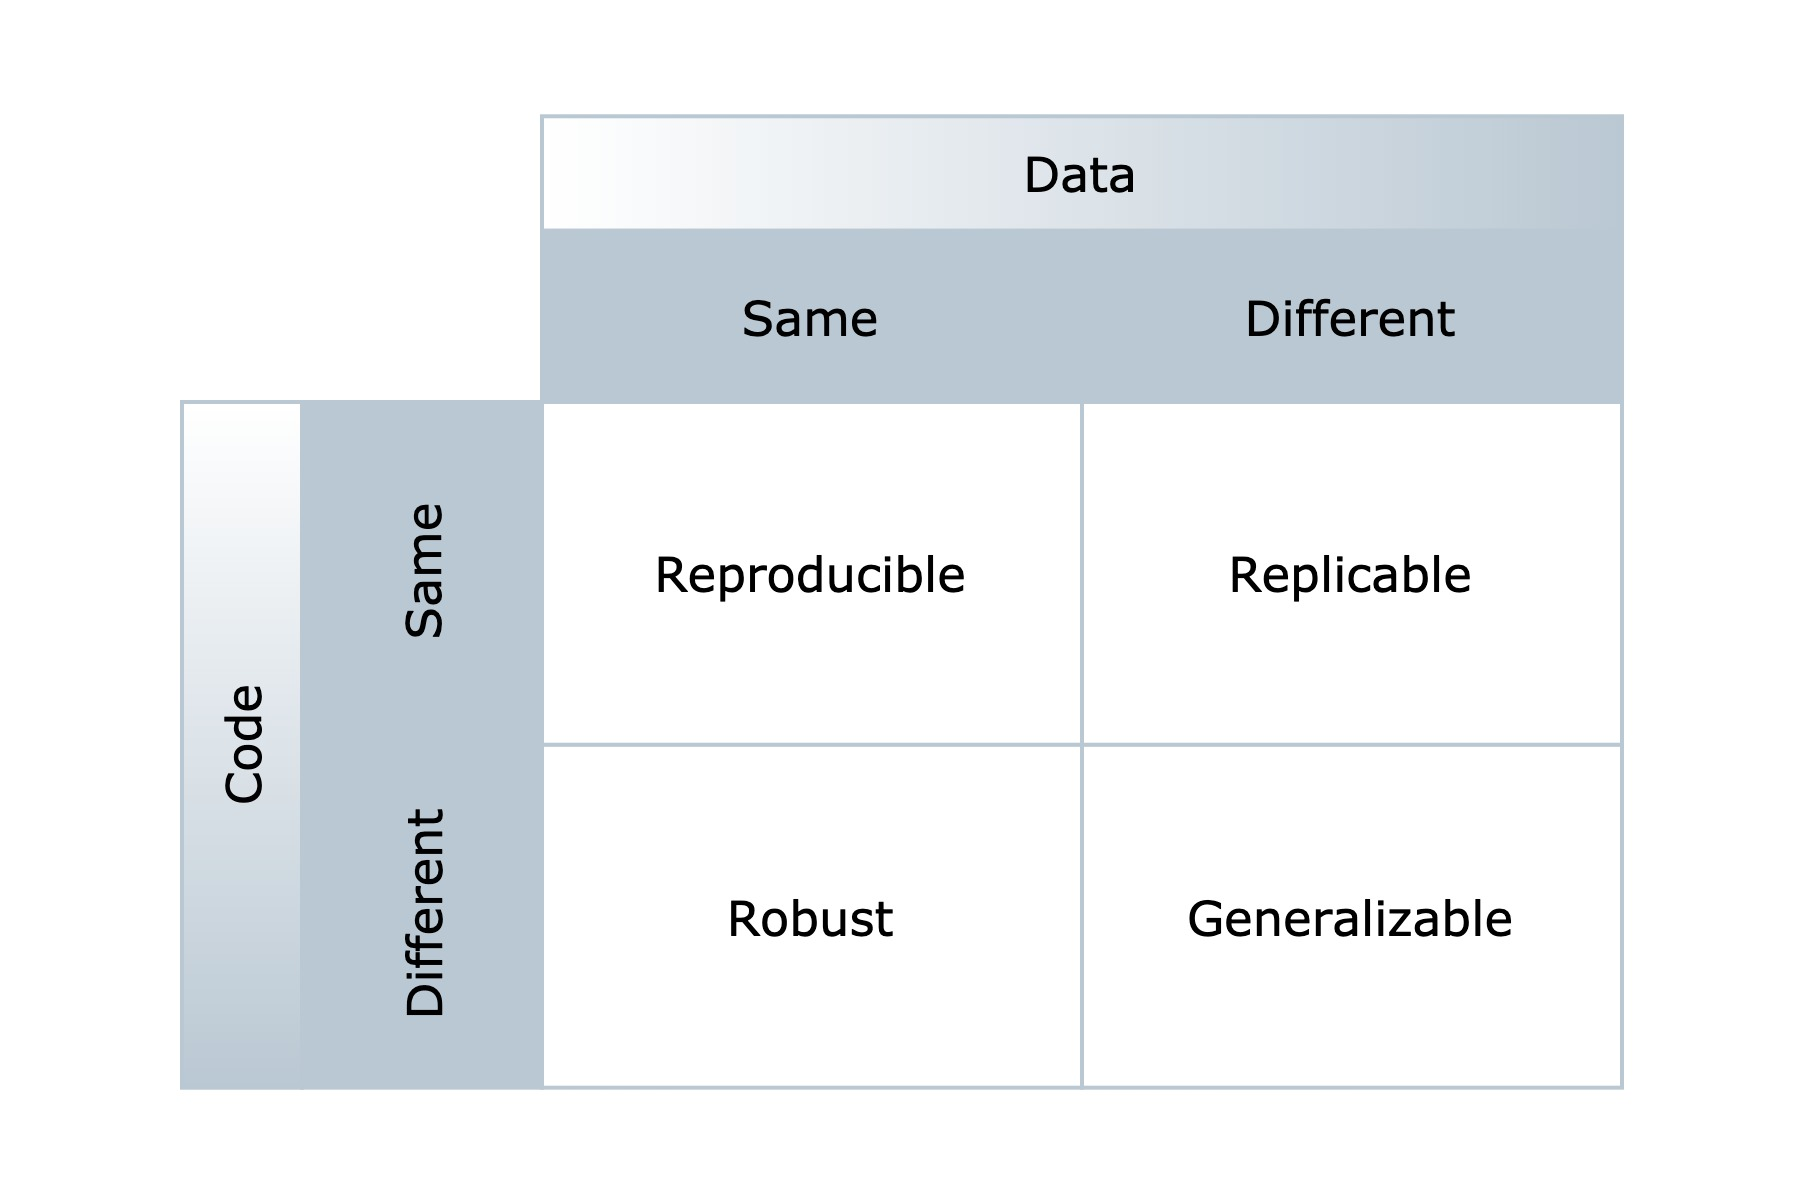
\includegraphics[width=0.60\textwidth]{figures/01ReproducibleReplicable.jpg}
    \caption{Reproducible, Replicable, Robust and Generalizable research reproduced from~\cite{whitaker_showing_2017}}
    \label{fig:ReproducibleReplicable}
\end{figure}

For achieving reproducibility, all the required information for re-doing the experiment should be available on the 
study report. For example, when collecting the initial data for the study, if the data is collected within a predetermined 
framework or it is being cured before being used, then all the related information needs to be included. For a machine learning 
problem, the same rule applies to data pre-processing, feature engineering, classification algorithm, result generation, 
performance metrics calculation and any other possible involved process.

A \textbf{replicable} study is the one that could re-generate the same results, if the same analytical tools are applied to a 
different set of data (relevant data being collected and cured through the same framework, distribution and method) and 
through the same environment.

A study is \textbf{robust}, if the same results could be achieved by applying different analysis (e.g. re-implementing the code 
in a different environment or using the same algorithm from a different well-recognized library) to the same set of data.

A \textbf{generalizable} study leads to the same results if a different analysis is applied to a different set of data 
(in such a way mentioned above). 

Figure~\ref{fig:ReproducibleReplicable} illustrates reproducible, replicable, robust and generalizable research in regards 
to data and analysis. If a study is not reproducible, then replicability, robustness and generalizability of that experiment 
could not be assessed. Through this study, our focus is on reproducible research as being addressed in this section.

\subsubsection{Method reproducibility, Result reproducibility, Inferential reproducibility}
Goodman et al [8] explain that the reproducibility and replicability definitions being provided by the U.S.National 
Science Foundation (NSF) \cite{cacioppo_social_2015}, do not provide a clear operational criteria for making a distinction 
in between these two concepts. Based on the published definitions, one can not draw a clear line in between what constitutes 
a successful reproduction or replication. To address the underlying construct of a reproducibility study, they suggest using 
three following terms instead of reproducibility. They believe these terms can make a more meaningful distinction in between 
various interpretations of reproducibility.

\textbf{Method reproducibility} is the ability to implement the original study experiment using the same data, analysis tools and 
through the same environment to obtain the same result. In definition and practice, it is the same as the original 
reproducibility term being defined in the last section.

\textbf{Results reproducibility} (previously defined as replicability) is the ability to re-generate the same results in a new 
(independent) study by following the same experimental procedures being provided in the original study on a new set of data.

\textbf{Inferential reproducibility} is the ability to achieve qualitatively similar conclusions from reanalysis or replication of 
the original study.

In our study, we address the methodological reproducibility of the problems with an imbalance datasets as being described in 
this section.

\subsubsection{Low, Medium and High Reproducibility}
According to the current standards (being placed to ensure the reproducibility of a claim) for a paper to be 
reproducible (adopted by conferences like NeurIPS \cite{pineau_improving_2020}), all the details of the study should be 
included in the submitted paper. Also, the data, programs and any involved  software needs to be submitted along with 
the study report. But sometimes due to some restrictions (e.g. confidentiality \cite{dwork_fienberg_2018}) submitting all 
the required materials are not possible. Thus, the “reproducible” term, can not describe how reproducible an experiment is. 
When it comes to older studies, this problem is even more visible as some involved materials are not accessible anymore.
 To address this problem~\cite{tatman_practical_2018} proposes three following terms by which the amount of 
 reproducibility could be expressed.

\textbf{Low reproducibility:} A low reproducible study is one that has only submitted the experiment report for the claim. 
The paper needs to contain all the correspondent details for an independent reproduction of the same experiment from scratch. 
The reproduced work needs to generate the same results.

\textbf{Medium reproducibility:} A study with medium level of reproducibility shares the codes and data along with the 
experiment report. The submitted data and code should permit an independent reproduction of the experiment leading to 
the same conclusion.

\begin{figure}[ht]
    \centering
    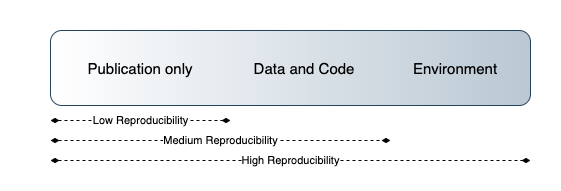
\includegraphics[width=0.90\textwidth]{figures/02HighLowReproducibility.jpg}
    \caption{Studies with Low, Medium and High degree of Reproducibility}
    \label{fig:LowHighReproducibility}
\end{figure}

\textbf{High reproducibility:} A study is highly reproducible if the environment information through which the experiment 
has been conducted, is also shared along with the data, code and the submitted paper. By definition, the environment 
includes all the libraries and dependencies necessary for a program to be run on a new machine. This level of reproducibility 
has been referred to as "linked and executable code and data" in \cite{peng_reproducible_2011}.

Figure~\ref{fig:LowHighReproducibility}, shows the reproducibility spectrum through which the above three terms 
could be addressed. In our study of classification problems with an imbalance dataset, we address the potential 
underlying issues of the studies with low degree of reproducibility and how those could lead to a wide range of 
results in reproduction.

\subsection{Reproducibility Crisis}
As being mentioned earlier in this section, the “reproducibility” term has been around for a while meaning that 
researchers were always concerned about the results of the studies in their domain of interest. We can track this 
back to the early 90s when John Claerbout in his book, "Earth Soundings Analysis" \cite{claerbout_earth_1992} 
claimed that few published results are reproducible in practice. 

\begin{figure}[ht]
    \centering
    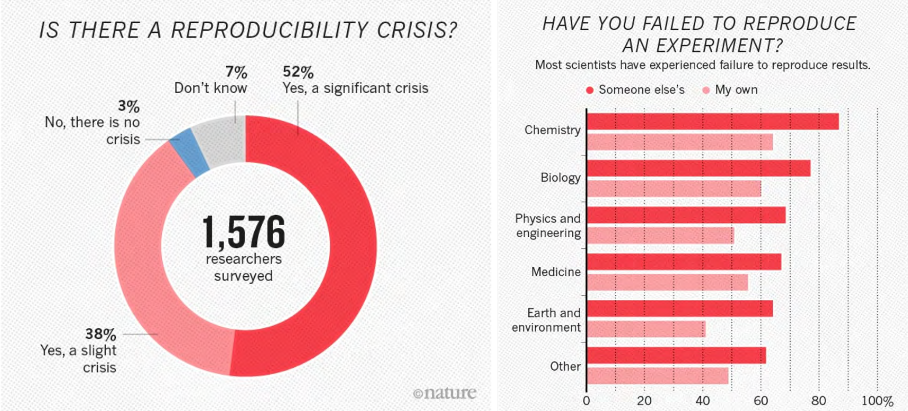
\includegraphics[width=0.90\textwidth]{figures/04NatureMagazine.png}
    \caption{Reproducibility crisis related results of the survey conducted by Nature in 2016 extracted 
    from~\cite{baker_1500_2016}}
    \label{fig:reproducibilityCrisis}
\end{figure}

With the emergence of disappointing results from large scale reproducibility projects in various domains, the term 
“Reproducibility crisis” gained currency in publications over the last decade (e.g. \cite{pashler_editors_2012}). 
In a study being conducted by the Nature journal in 2016 \cite{baker_1500_2016}, more than 70\% of surveyed scientists 
reported failure in their attempt to reproduce another scientist's experiments, and more than half (52\%) believed 
that science is facing a “reproducibility crisis”. The cause of the problem covers a wide range of subjects from 
pressure to publish and selective reporting to poor analysis. Most of the researchers believed that failure to reproduce 
published results does not mean that the result is probably wrong, and most say that they still trust the published 
literature. Figure~\ref{fig:reproducibilityCrisis} shows reproducibility crisis related  results of the survey 
conducted by Nature in 2016 .

On the same subject in machine learning, Nicolas Rougier, a computational neuroscientist says “I think people 
outside the field might assume that because we have code, reproducibility is kind of 
guaranteed” but "far from it" he said at France's National Institute for Research in Computer Science 
and Automation in Bordeaux~\cite{hutson_artificial_2018}. 
One of the common problems is that due to some restrictions (e.g. confidentiality), 
the dataset or source code used in the study is not open-sourced.  For example in a reproducibility study on 400 
presented papers at two top AI conferences conducted by Odd Erik Gundersen, 6\% of the presenters had released 
their codes, third of them had shared their data, and 50\% had shared their pseudocodes \cite{gundersen_state_2018}.

Through recent years, the results of similar studies across different domains, have raised great concerns in the scientific 
community leading to various works providing reproducibility-related lexicons, guidelines, and platforms for measuring and 
improving the reproducibility of the research results. In a move aimed at providing reproducible research, some conferences 
even put new mandates in places for submitting the publications 
\cite{pineau_improving_2020,goodman_what_2016,tatman_practical_2018}. In this work, we address the potential 
reproducibility-related issues of the classification problems with imbalanced datasets. 

\subsection{Reproducibility-related works}
Throughout the past decade, reproducibility-related studies have received a notable amount of attention in the 
scientific community. Figure~\ref{fig:publications} shows the publications recorded in the Scopus that have, in the title or abstract, 
at least one of the reproducibility-related expressions \cite{goodman_what_2016}. The studies have been conducted in 
various domains from different perspectives to define the terms, address the cause of the problem, create frameworks, 
platforms, guidelines and mandated to encourage reproducible research in practice. In this section, we will mention 
some of the related works in the field.

Around the same time when Claerbout claimed that few published results are reproducible~\cite{claerbout_earth_1992}, 
a computer scientist, Donald Knuth, introduced 
the concept of Literate Programming \cite{knuth_literate_1984}. In Literate Programming, computer code is embedded within 
the program's documentation making it more understandable for humans. The consolidated standards of reporting trials 
or consort [\linkto{http://www.consort-statement.org}], published a set of guidelines In 1996 to fix problems associated 
with inadequate reporting of randomized controlled trials.

In 2004, the International Committee of Medical Journal [\linkto{http://www.icmje.org}] announced that they would not publish a 
clinical trial without registration. The updated publication's criterias includes conditions like 
“Manuscripts submitted to ICMJE journals that report the results of clinical trials must contain a data sharing statement”. 
In a move towards reproducible research, the Journal of Biostatistics [\linkto{https://academic.oup.com/biostatistics}] began 
marking accepted papers based on the standards of reproducibility. also encouraged reproducible practices of authors 
submissions. For example, D means the study data is freely available, A C means the code is available and R means the 
paper is reproducible. 

\begin{figure}[ht]
    \centering
    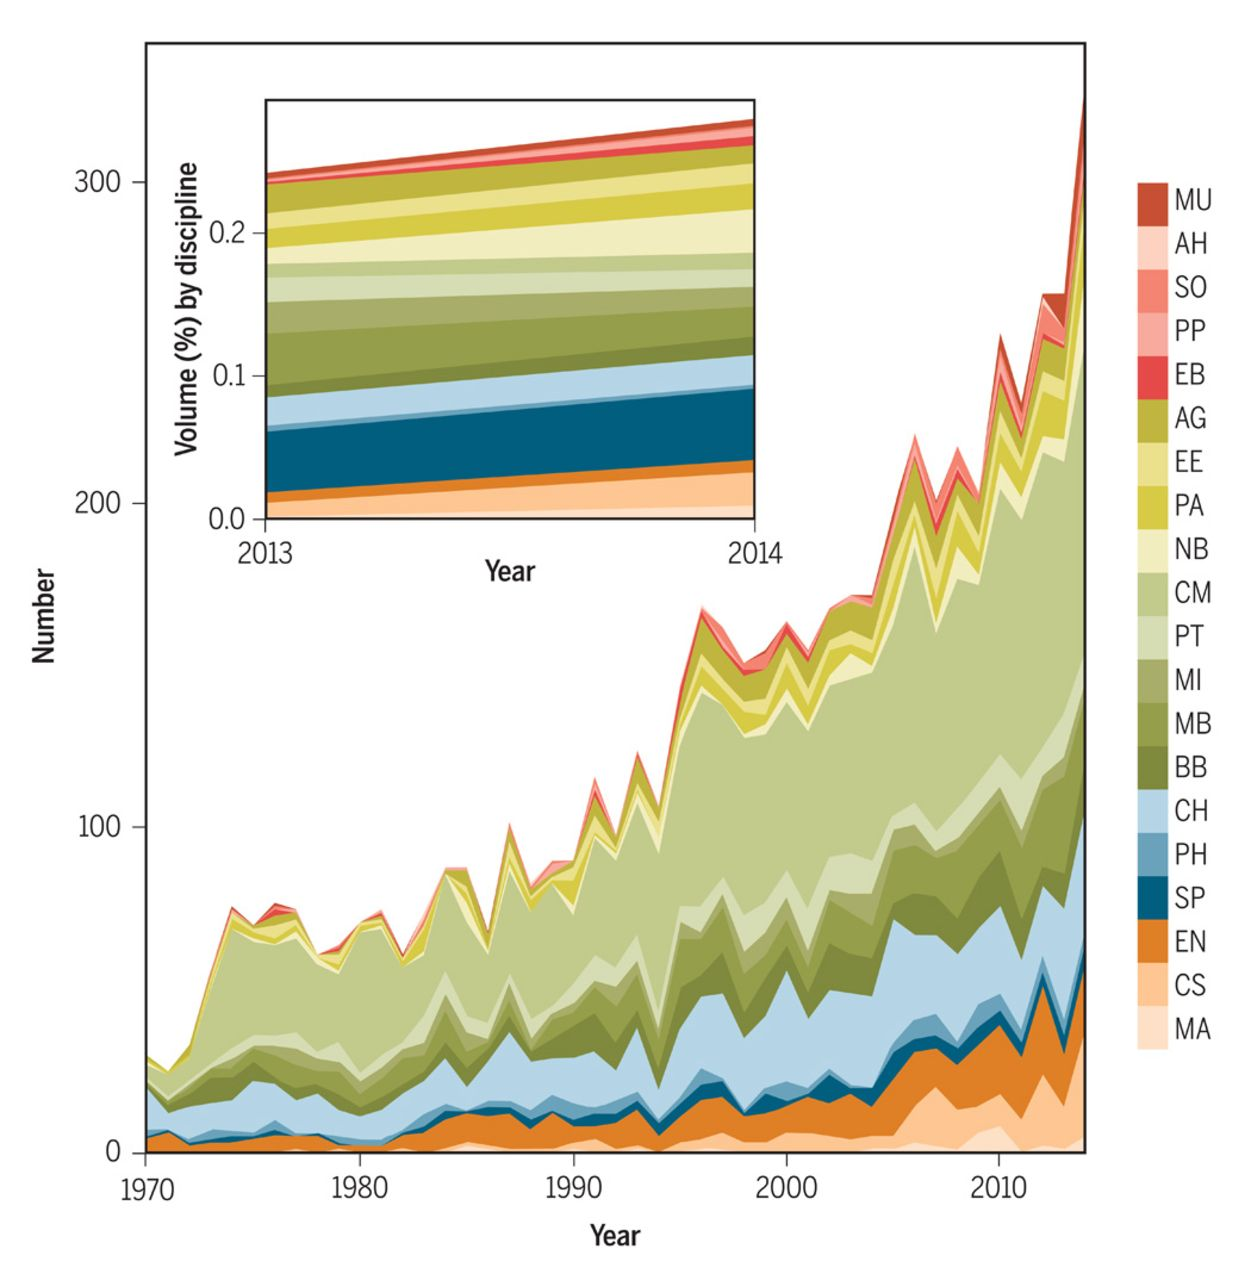
\includegraphics[width=0.60\textwidth]{figures/03ReproducibilityPubTimeline.jpg}
    \caption{ publications recorded in the Scopus that have, in the title or abstract, 
    at least one of the reproducibility-related expressions extracted from~\cite{goodman_what_2016}}
    \label{fig:publications}
\end{figure}

In research on 500 research papers in 2011 \cite{alsheikh-ali_public_2011},  30\% of the submitted papers did not adopt 
any data sharing policy. Among the ones who adhered to the data sharing instructions, 91\% deposited only the 
specific required data type and 9\% made the full primary raw data accessible online. The Open Science Collaboration 
in 2015 \cite{open_science_collaboration_estimating_2015} announced that only 30-50 percent of the results being taken 
from more than 100 studies were reproducible. U.S. National Science Foundation (NSF) \cite{cacioppo_social_2015} in 2015, 
addresses the reproducibility problem providing definitions for reproducibility, replicability, robustness and generalizability.  

ASCB’s survey on reproducibility in 2015 \cite{ascb_ascb_2015} showed that almost 70\% of the questioned researchers 
were unable to replicate the results of studies they were interested in. Nature journal in 2016 \cite{baker_1500_2016}, 
addresses the “reproducibility crisis” by conducting a survey. The study showed that more than 70\% of surveyed 
scientists reported failure in their attempt to reproduce another scientist's experiments.  In 2106, Mark D. Wilkinson et al 
\cite{wilkinson_fair_2016} wrote a paper on FAIR principles, providing guidelines for implementing Findable, 
Accessible, interoperable and Reusable research in practice.

Steven N. Goodman et al in 2016~\cite{goodman_what_2016} published a paper suggesting new terms for reproducibility. 
They believed the underlying construct of the reproducibility studies could be addressed by using these new terminologies. 
In 2017, Babatunde K. Olorisade et al~\cite{olorisade_reproducibility_2017}, published a paper on practicing reproducibility 
in machine Learning studies by providing an example in the text mining domain. Through the same year 
Hans E. Plesser~\cite{plesser_reproducibility_2018} also published a paper in “Frontiers in Neuroinformatics” 
clearing up on the various in-use definitions of the reproducibility-related term in the field.

In 2018, Joelle Pineau et al \cite{pineau_improving_2020} provided guidelines for improving reproducibility in 
machine learning research. She also published a “The Machine Learning Reproducibility Checklist”  designed to be used 
simultaneously with the ML code submission checklist for NeurIPS. In his paper, Rachael Tatman~\cite{tatman_practical_2018} 
provided a new taxonomy for reproducibility for machine learning research in 2018 by which the amount of reproducibility 
could be expressed. 

In 2019, Andrew L. Beam et al~\cite{beam_challenges_2020} published a paper on the reproducibility 
of the machine learning models in health care discussing the unique challenges for the problems using machine learning 
models to predict the outcome. Since a machine learning model should be reproduced, and ideally replicated, before it 
is deployed in a clinical setting, they highly encourage adopting reproducible research practices for the studies in 
this field. Through the same year, Matthew B.A. McDermott et al~\cite{mcdermott_reproducibility_2019} 
also published a paper on reproducibility in machine learning for health (ML4H) providing a comparison between the 
available amount of reproducibility in the field and other machine learning-based domains of studies. 
They also discuss the causes of the problem, the unique challenges associated with the problems in this field 
(e.g. confidentiality) providing guidelines over how to improve reproducibility considering the current challenges.

The scientific community has also initiated and developed various softwares and platforms (such as 
scikit-learn ~\cite{pedregosa_scikit-learn_2018}, R~\cite{chambers_software_2008},  etc.) for software development in general and 
statistical computing in specific (in our case) through the reproducible research framework. All these cumulative 
efforts have been done in an aim to provide all the researchers with free, well-documented and publicly accessible 
softwares leading to creation of standard practices and reproducible studies.
